\documentclass[a4paper,11pt]{article}
\usepackage{graphicx}
\usepackage{amsmath}
\usepackage{hyperref}
\usepackage{geometry}
\usepackage{natbib}
\usepackage{project}
\usepackage{tikz}
\usetikzlibrary{positioning, shapes.geometric, arrows}

\geometry{margin=1in}

\begin{document}

\section{Questions}
\begin{itemize}
    \item How do changes in atmospheric \(\text{CO}_2\) concentrations correlate with changes in sea level rise over time?
    \item Is there a correlation between rising mean surface temperatures and land cover changes?
\end{itemize}

\section{Data Sources}
\subsection{Description of Data Sources}
\begin{itemize}

\item \textbf{Dataset 1: Annual Surface Temperature Change}
    
This data source provides the mean surface temperature change for the period 1961–2021 for each country. It uses temperatures from 1951 and 1980 as a baseline. \cite{dataset1} 
    
\item \textbf{Dataset 2: World Monthly Atmospheric \(\text{CO}_2\) Concentrations}

In this data source, world-wide average concentrations of \(\text{CO}_2\) are present, which have been observed on a monthly basis since 1958. \cite{dataset2}
    
\item \textbf{Dataset 3: Change in Mean Sea Levels}

The indicator provided in this data source is global sea level rise for different seas and oceans, observed monthly since 1993. \cite{dataset3}

\item \textbf{Dataset 4: Land Cover Altering Indicator}

This data source looks at the changes in land cover over time from 1992 to 2020 for each country. The indicator is grouped into categories on the basis of climate influence: altering, regulating, and neutral. \cite{dataset4}

\end{itemize}

\subsection{Data Structure and Quality}
\begin{itemize}
    \item \textbf{Annual Surface Temperature Change} The data is structured in a time series for each country in a horizontal manner. Temperature change is in degree-Celsius units. The main columns to use are country, iso3 (i.e., country code mapping required for generating maps), and indicator values for all the years. At most, 8\% of the data in one of the years is unobserved, which is fine as that can be imputed with zeros.

    \begin{figure}[ht!]
        \centering
        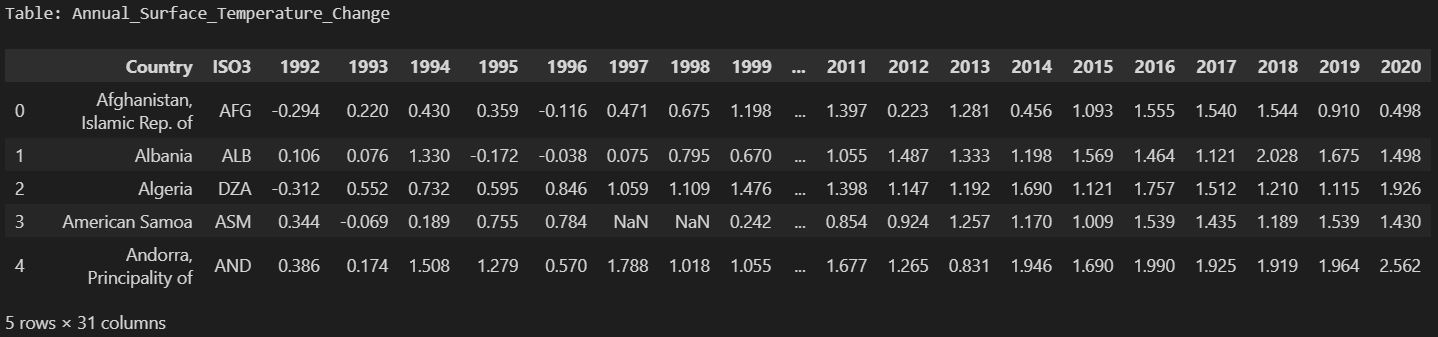
\includegraphics[width=0.9\textwidth]{pictures/atmos.png}
        \caption{First 5 rows of annual surface temperature change dataset.}
        \label{fig:dataset1}
    \end{figure}
    
    \item \textbf{World Monthly Atmospheric \(\text{CO}_2\) Concentrations} This indicator of \(\text{CO}_2\) concentration is structured in a global time series with a monthly frequency. The main columns are date and value. The indicator value is expressed in parts per million (ppm). Nulls are 0\% in this dataset.

    \begin{figure}[ht!]
        \centering
        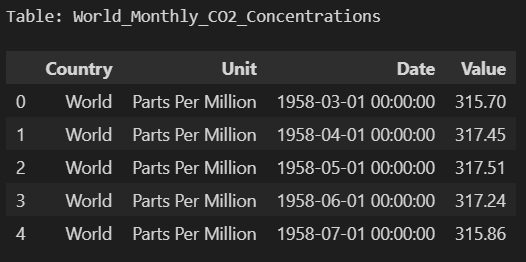
\includegraphics[width=0.4\textwidth]{pictures/co2.png}
        \caption{First 5 rows of world monthly atmospheric \(\text{CO}_2\) concentrations dataset.}
        \label{fig:dataset2}
    \end{figure}

    \item \textbf{Change in Mean Sea Levels} In this dataset main columns are measure, date and value in millimeters. It is again a time series observed with a monthly frequency but it is categorized into major seas and oceans in measure column. There are 0\% nulls in this dataset.

    \begin{figure}[ht!]
        \centering
        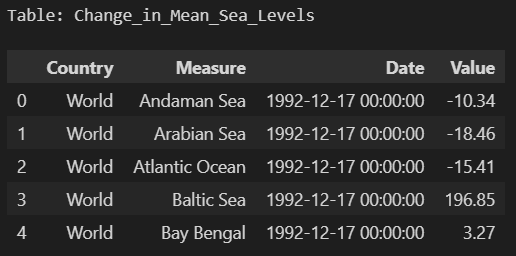
\includegraphics[width=0.4\textwidth]{pictures/sea.png}
        \caption{First 5 rows of change in mean sea levels dataset.}
        \label{fig:dataset3}
    \end{figure}

    \item \textbf{Land Cover Altering Indicator} This dataset is the land cover estimation of each country into three main categories of climate influence: altering, regulating, and neutral. Annual values are in a time series for each country in horizontal manner. At most 0.3\% of the data in one of the years is unobserved, which is fine as that can be imputed with zeros.

    \begin{figure}[ht!]
        \centering
        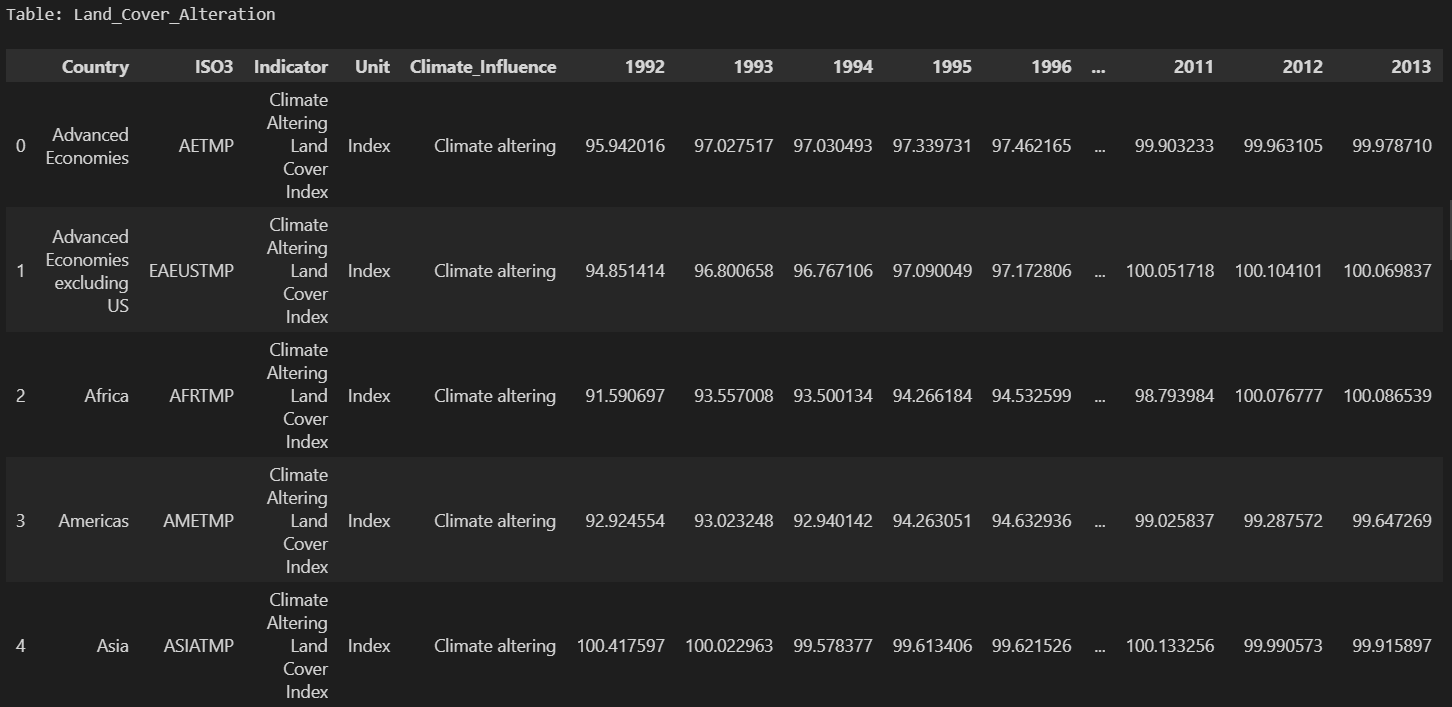
\includegraphics[width=0.6\textwidth, height=0.2\textheight]{pictures/land.png}
        \caption{First 5 rows of land cover altering indicator dataset.}
        \label{fig:dataset4}
    \end{figure}


\end{itemize}

\subsection{Licenses and Permissions}
The data sources are publicly available on \href{https://climatedata.imf.org/}{IMF} under open-data licenses. Detailed license information can be found at:
\href{https://www.imf.org/external/terms.htm}{License}

\section{Data Pipeline}
The data pipeline has three main modules: extractor, transform, and loader. Each of the modules has their respective functions.
First \texttt{extract\_csv} from extractor module is used to extract the data source from URL, then \texttt{delete\_columns} from transform module deletes the list of useless columns specified for every dataset, then a flag of "date\_column" is present in configs which only applies \texttt{standardize\_date\_column} to standardize the date format across necessary datasets, then renaming of the date columns is done using \texttt{rename\_year\_columns} function, it is only triggered for those datasets where flag  of "rename\_year\_columns" is equals to true, once all the transformations have been applied, dataset is then loaded to sqlite database using \texttt{load\_df\_to\_sqlite} from loader module.


\begin{figure}[h]
    \centering
    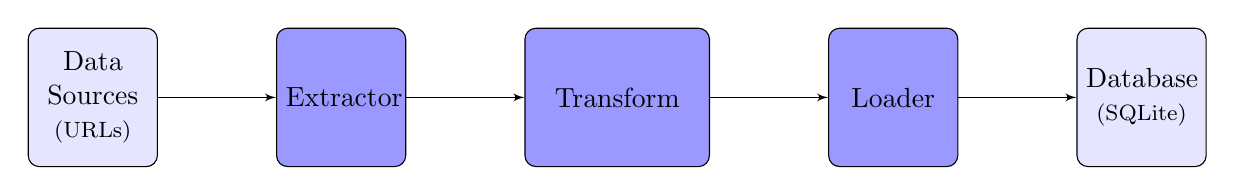
\begin{tikzpicture}[node distance=1.5cm and 1.5cm, auto]
        % Styles
        \tikzstyle{smallblock} = [rectangle, draw, fill=blue!10, 
            text width=4em, text centered, rounded corners, minimum height=5em]
        \tikzstyle{block} = [rectangle, draw, fill=blue!40, 
            text width=4em, text centered, rounded corners, minimum height=5em]
        \tikzstyle{largeblock} = [rectangle, draw, fill=blue!40, 
            text width=6em, text centered, rounded corners, minimum height=5em]
        \tikzstyle{line} = [draw, -latex', shorten >=0pt, shorten <=0pt]

        % Nodes
        \node [smallblock] (source) {Data Sources \\ \footnotesize (URLs)};
        \node [block, right=of source] (extractor) {Extractor};
        \node [largeblock, right=of extractor] (transform) {Transform};
        \node [block, right=of transform] (loader) {Loader};
        \node [smallblock, right=of loader] (database) {Database \\ \footnotesize (SQLite)};

        % Connections
        \path [line] (source) -- (extractor);
        \path [line] (extractor) -- (transform);
        \path [line] (transform) -- (loader);
        \path [line] (loader) -- (database);
    \end{tikzpicture}
    \caption{ETL Pipeline Diagram}
    \label{fig:etl_pipeline}
\end{figure}


\section{Result and Limitations}
Output datasets of the pipeline for all data sources are stored in sqlite database as tables as it was faster and easier to handle as a collective database, The pipeline is coded in a way that data quality dimensions were of the upmost priority and that the output datasets of the pipeline 
\begin{itemize}
    \item reflect the real word and are correct indicators
    \item contain all necessary information which is required to answer selected questions
    \item are consistent in their formats
    \item time period of datasets are appropriate and intersecting
    \item presentation of the datasets aligns with the requirements of the questions need to be answered
\end{itemize}

Annual surface temperature change and land cover altering indicator can be compared and checked for correlation and similarly the other two datasets can be compared. The only limitation is in the sea level dataset where the measure column is not friendly to be mapped on the world map for oceans and seas and no code mappings were found for them.

\bibliographystyle{plain}
\bibliography{references}

\end{document}
